\chapter{Результаты проведённых расчётов} \label{ch3}


В данном разделе представлены результаты расчётов. Получены первые пять собственных частот и форм рассматриваемого изделия (рис. \ref{fig:mod1}-\ref{fig:mod5}).

\begin{figure}[H] 
	\center
	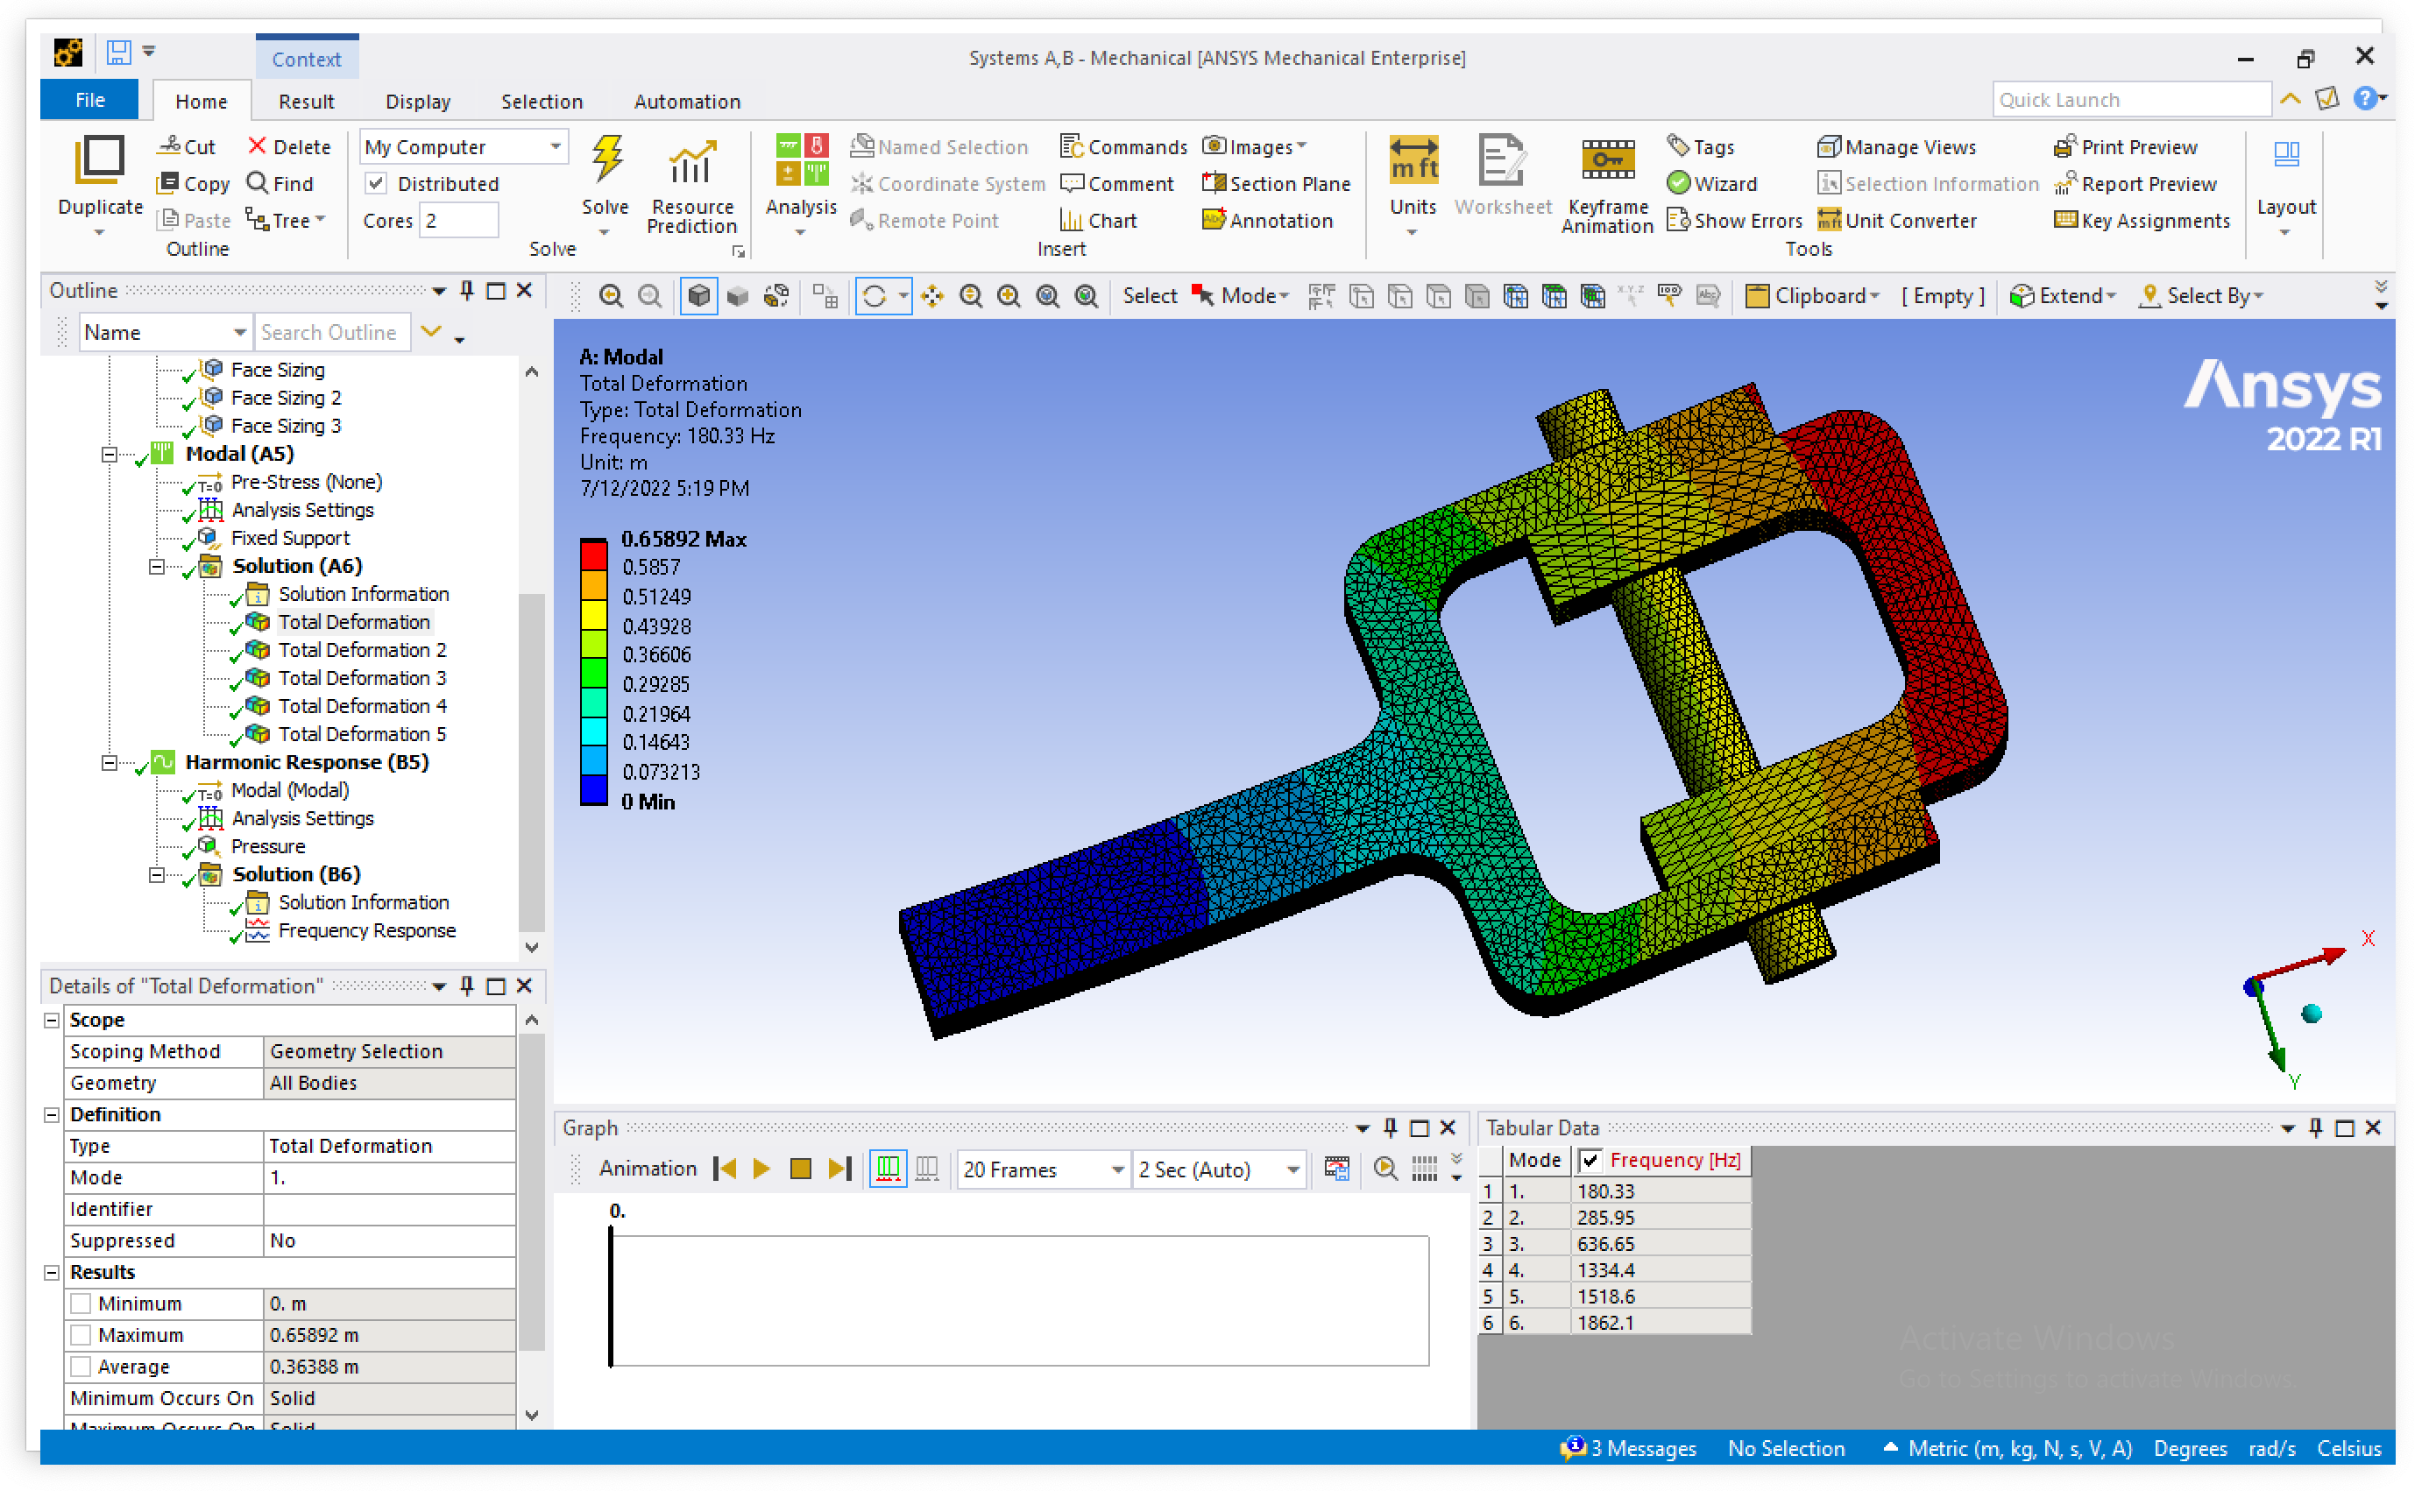
\includegraphics[width=.9\textwidth]{images/mod1.png}
	\caption{Деформации при первой собственной частоте (преимущественно вдоль оси Oy)}
	\label{fig:mod1}
\end{figure}

\begin{figure}[H] 
	\center
	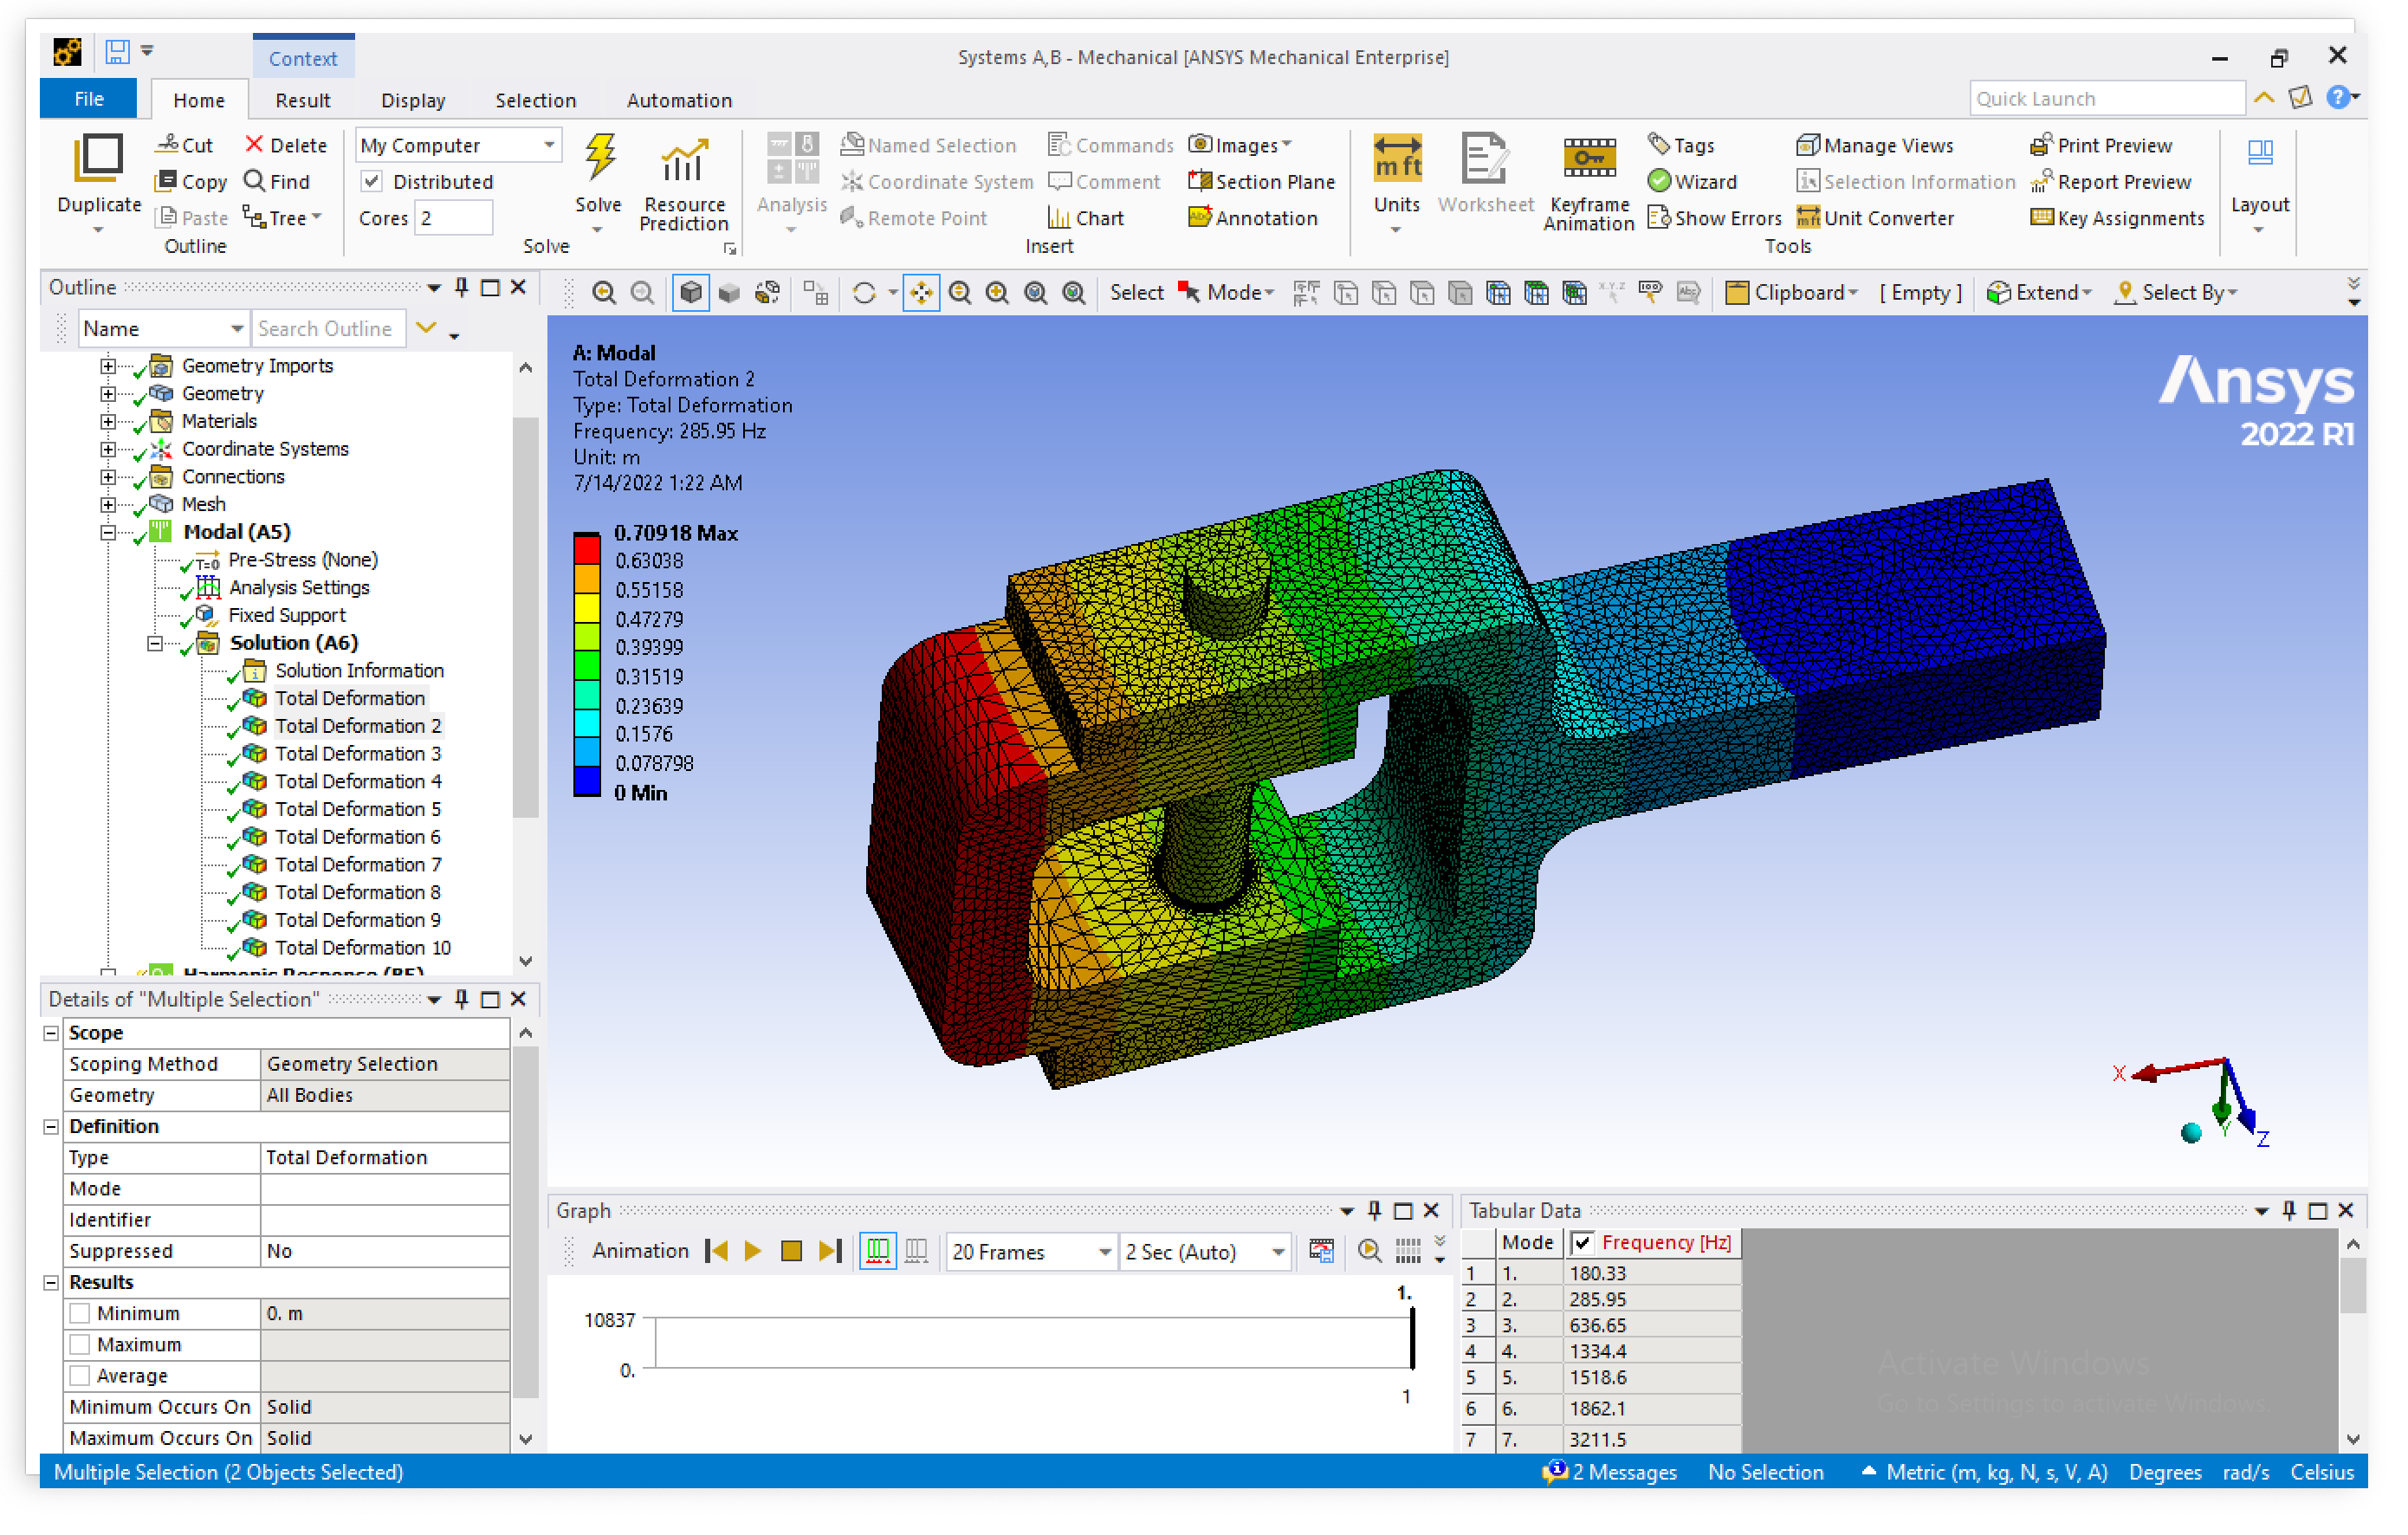
\includegraphics[width=.9\textwidth]{images/mod2.png}
	\caption{Деформации при второй собственной частоте (преимущественно вдоль оси Oz)}
	\label{fig:mod2}
\end{figure}

\begin{figure}[H] 
	\center
	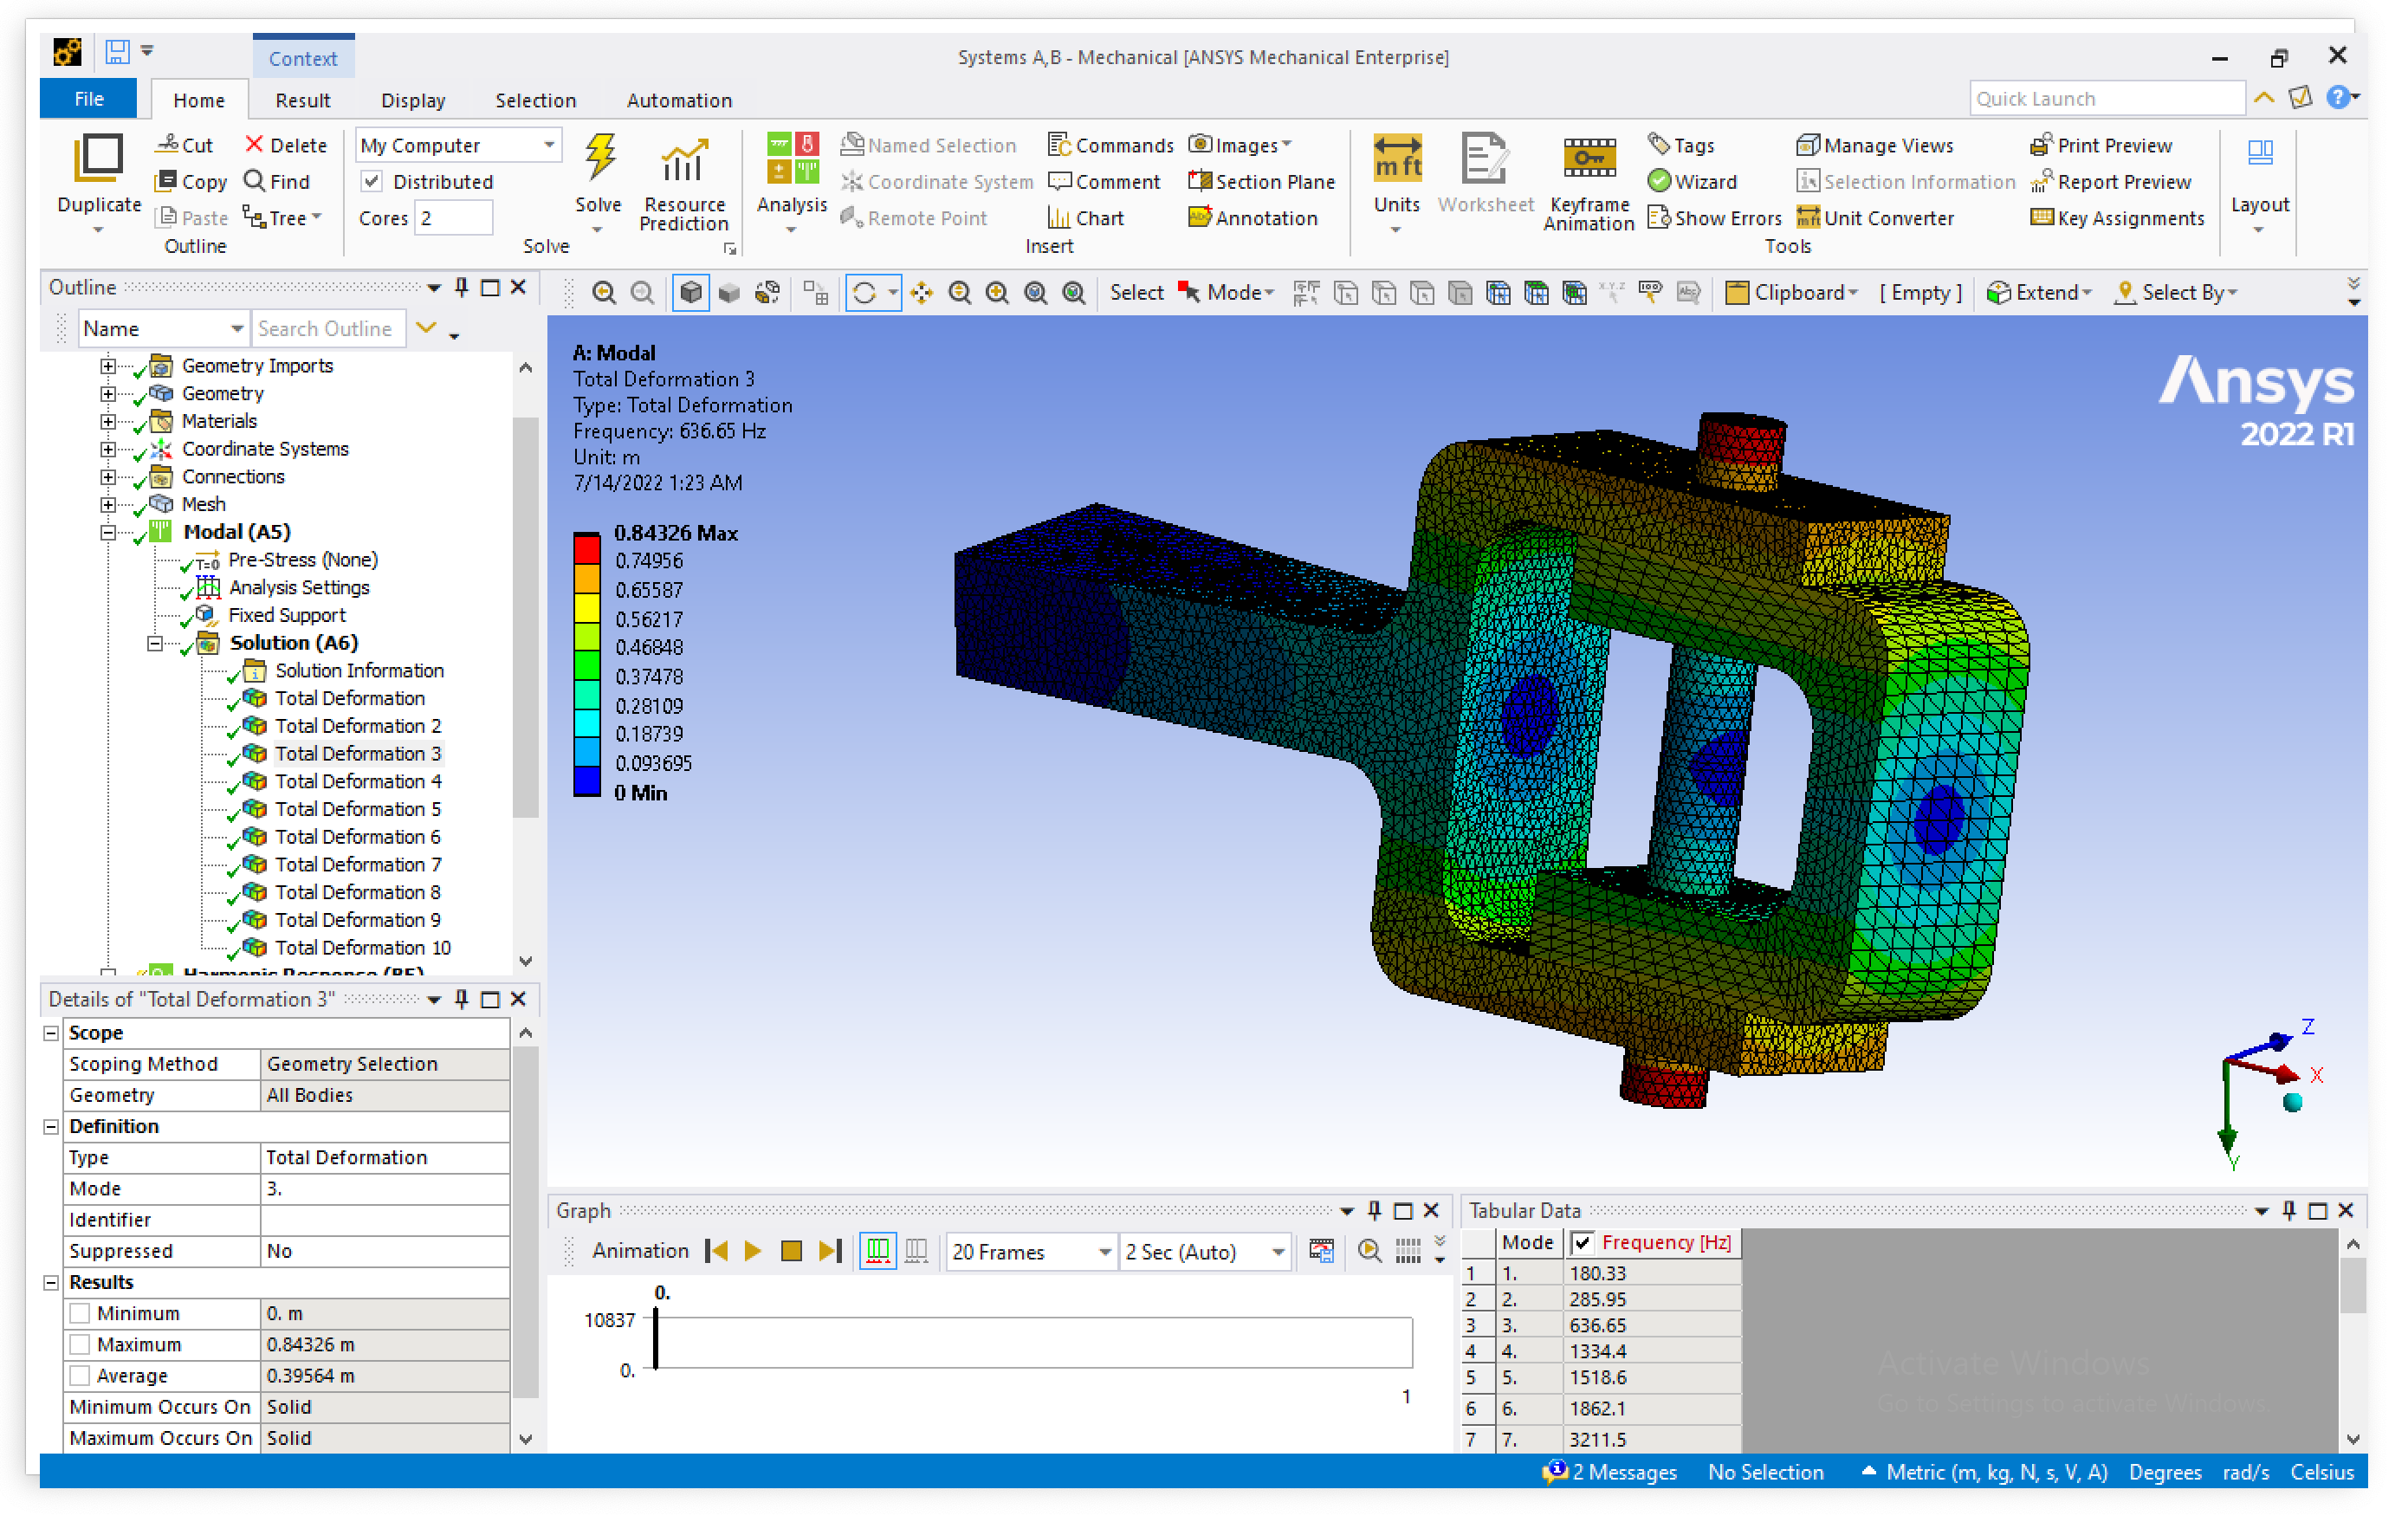
\includegraphics[width=\textwidth]{images/mod3.png}
	\caption{Деформации при третьей собственной частоте (преимущественно вдоль осей Ox и Oy)}
	\label{fig:mod3}
\end{figure}

\begin{figure}[H] 
	\center
	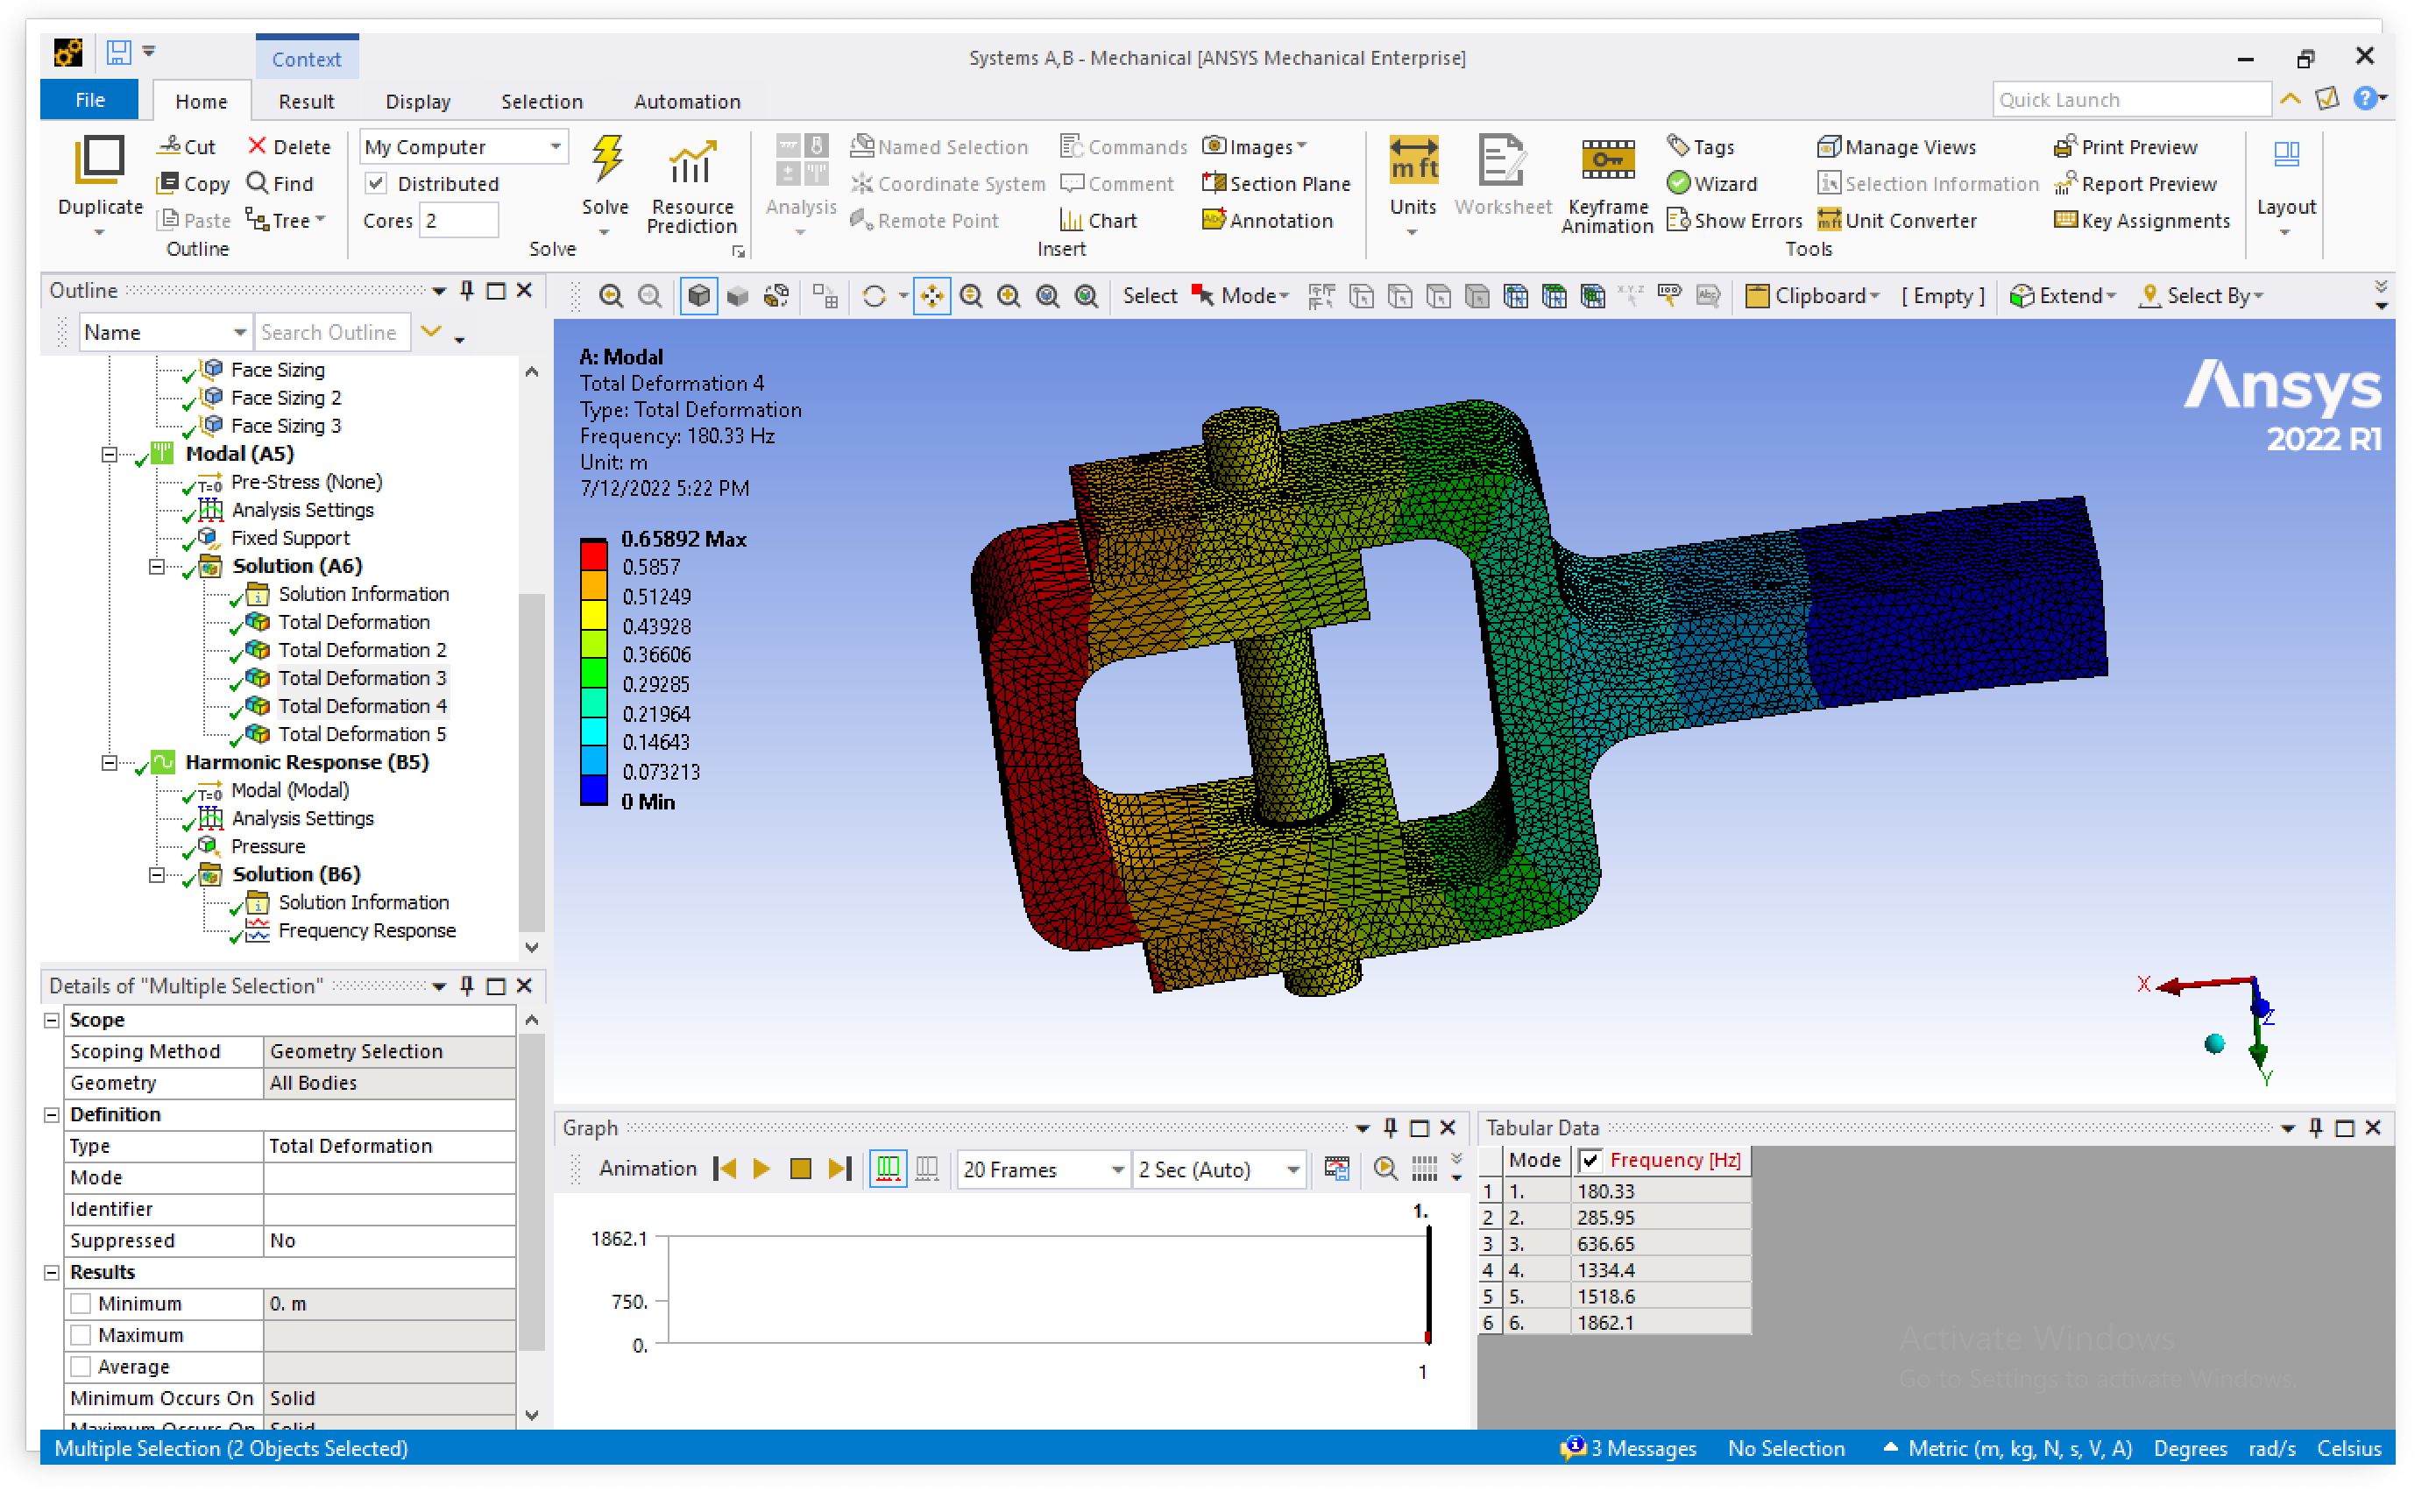
\includegraphics[width=\textwidth]{images/mod4.png}
	\caption{Деформации при четвёртой собственной частоте (преимущественно вдоль оси Oy)}
	\label{fig:mod4}
\end{figure}

\begin{figure}[H] 
	\center
	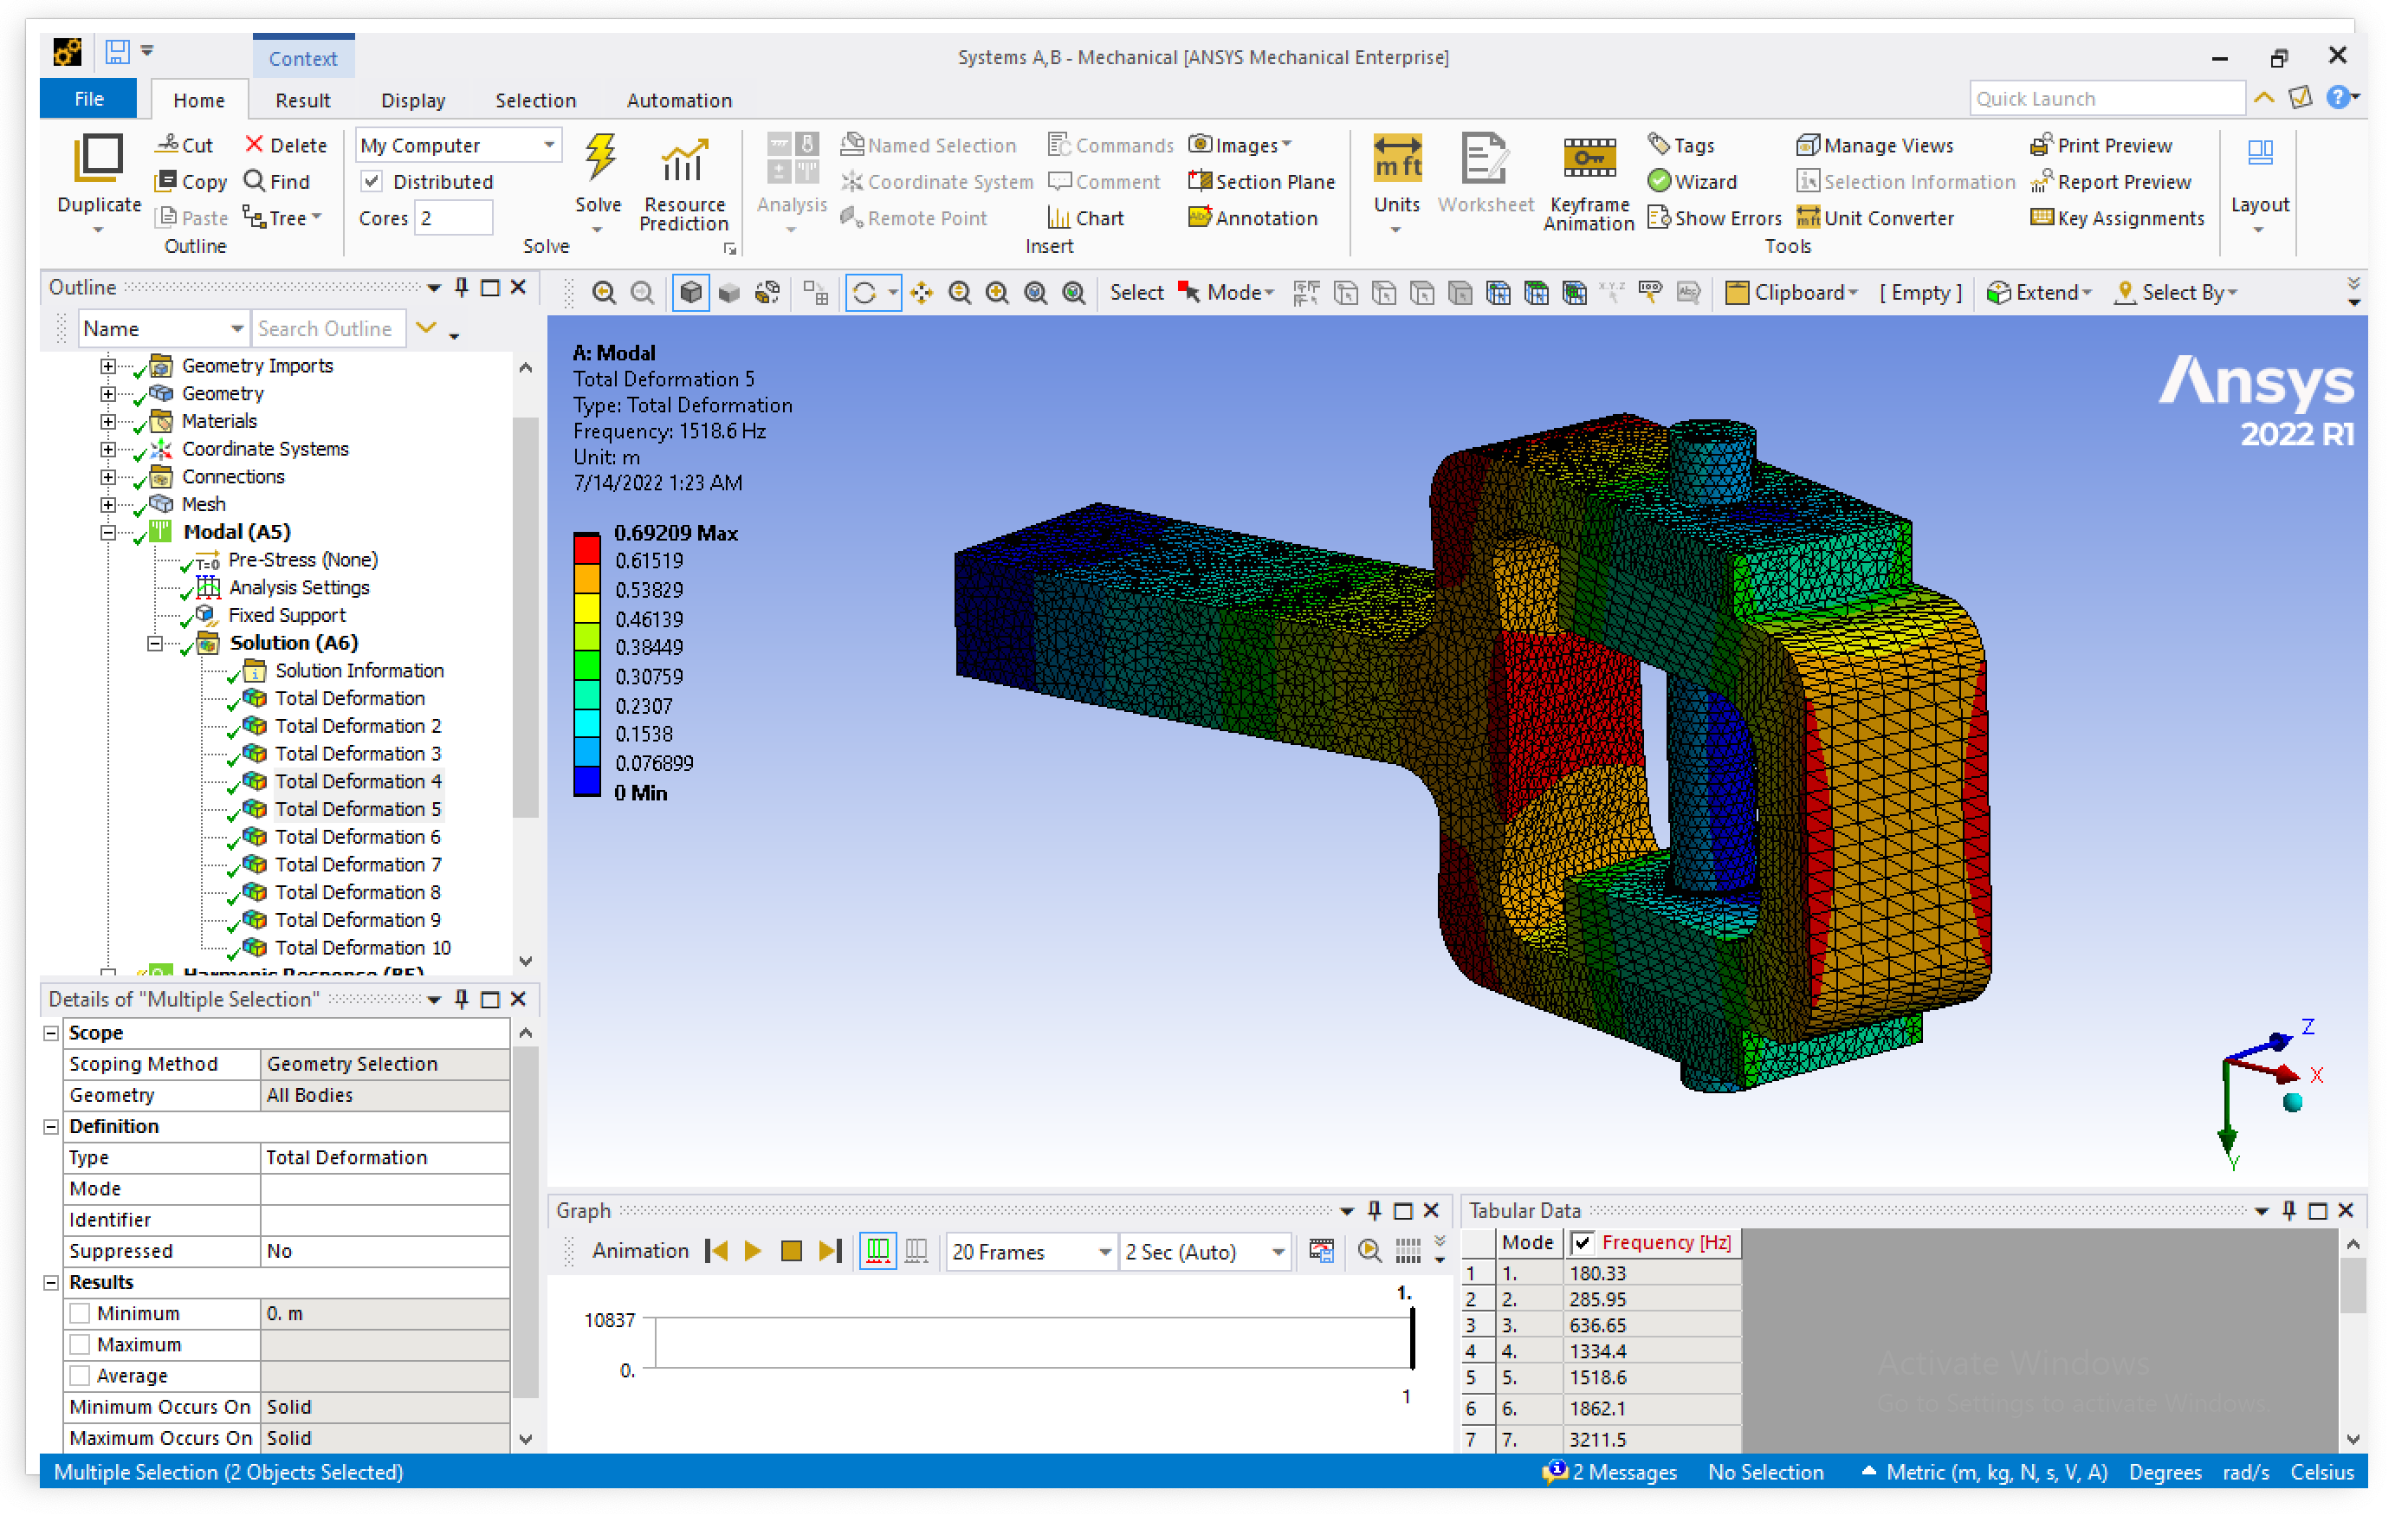
\includegraphics[width=\textwidth]{images/mod5.png}
	\caption{Деформации при пятой собственной частоте (преимущественно вдоль осей Ox и Oz)}
	\label{fig:mod5}
\end{figure}


Из полученных собственных частот и форм возможно прогнозировать, при каких частотах вибрации следует избегать эксплуатацию рассматриваемого изделия. Значения этих частот для данной геометрии и материала изделия представлены на рис. \ref{fig:frequency_tabular}.

\begin{figure}[H] 
	\center
	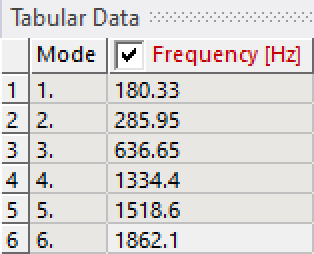
\includegraphics[width=.33\textwidth]{images/frequency_tabular.png}
	\caption{Собственные частоты}
	\label{fig:frequency_tabular}
\end{figure}

